Figure \ref{fig:siso-channels} shows the frequency response of one realization of multipath FF and FS channel based on the same tap delays and gains.

\begin{figure}
  \centering
  \subfigure[FF channel]{
    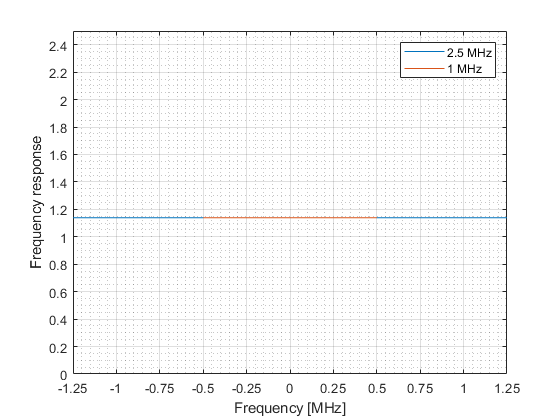
\includegraphics[width=0.48\textwidth]{siso_frequency_flat_channel}}
  \subfigure[FS channel]{
    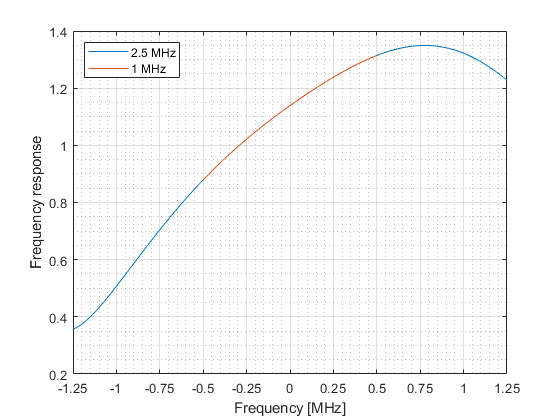
\includegraphics[width=0.48\textwidth]{siso_frequency_selective_channel}}
  \caption{Frequency response of the SISO FF and FS channels}\label{fig:siso-channels}
\end{figure}

In the R-E region, the rightmost point of each curve indicates the maximum achievable rate with zero harvested DC current. It corresponds to WIT where all transmit power is allocated to the modulated information waveform by water-filling algorithm with $\rho  = 0$. Note that the x-axis here refers to per-subband rate which is normalized w.r.t. bandwidth. Since the power budget is fixed, each subband indeed receives less power as $N$ increases. Therefore, the total capacity increases but the rate achieved by each subband indeed decreases. On the other hand, the leftmost point corresponds to the maximum output DC current with zero information rate, which is realized by allocating all power to the multisine waveform with $\rho  = 0$ (WPT). 

Nevertheless, the discrete rate constraint in WIPT optimization problem \ref{eqn:original_target} -- \ref{eqn:original_rate_constraint} prevents the solutions from achieving the absolute WIT points. Therefore, we performed individual WIT and combine the results to obtain the R-E plots. Also, the rate achieved by a certain solution can be slightly larger than the requirement, as the current gain of another iteration can be negligible (smaller than $\varepsilon$). 